\section{Design}
The problem this project tries to solve, revolves around tranferring data 
between research stations and the MiG. Its intended design is described below.

\subsection{Surrounding systems}

The system is supposed to interface with different entities, these are the
surrounding systems described below. The first system encountered is the user
storage medium, these typically provide either USB or FireWire interfaces,
secondly the system is supposed to interface with the MiG.

\paragraph{User storage device} are expected to typically be USB hard disks. 
This is expected based on the availability and their ease of use.

\paragraph{MiG} is providing the interface to the storage units, where the
system is supposed to upload the files to. 

MiG is a grid computing middleware, acting as the broker between users and
resources(CPU, storage, applications).

\textit{ ADD MORE }

\subsection{Overall design goals}

The solution focuses on two key aspects, authentication and temporary
autorisation and transfer of data. These two aspects represent their own 
sub-system which are designed independently, but with eachother in mind.

\paragraph{Data transfer} the data being transferred has a high price, it is
therefore vital to the system that the stored data exactly matches what was
originally recorded. Another point regarding transfer is the size of the
recorded data, it is expected that the system will move terabytes of data
between itself and MiG, this has to happen in a timely-manner.

The data transfer has these two factors as criteria for succes, reliability and
speed.

\paragraph{Authentication} is for the system the process of identifying itself
as the scientist wanting to upload data, furthermore the system needs to
authorize itself to allow the upload on behalf of the user. The currently
employed security model for MiG, has many advantages and is as secure as can
get while maintaining the MiG principles.

\subsection{List of requirements}

\subsection{Logic design}
The logical design of the system is shown in Figure \ref{fig:overall_design},
and futher expanded upon in this section.

The design depicts MiG as having two seperate entties, these are to be seen as
one. The seperation is mainly concerned with seperation of concerns.

\begin{figure}[h]
\centering
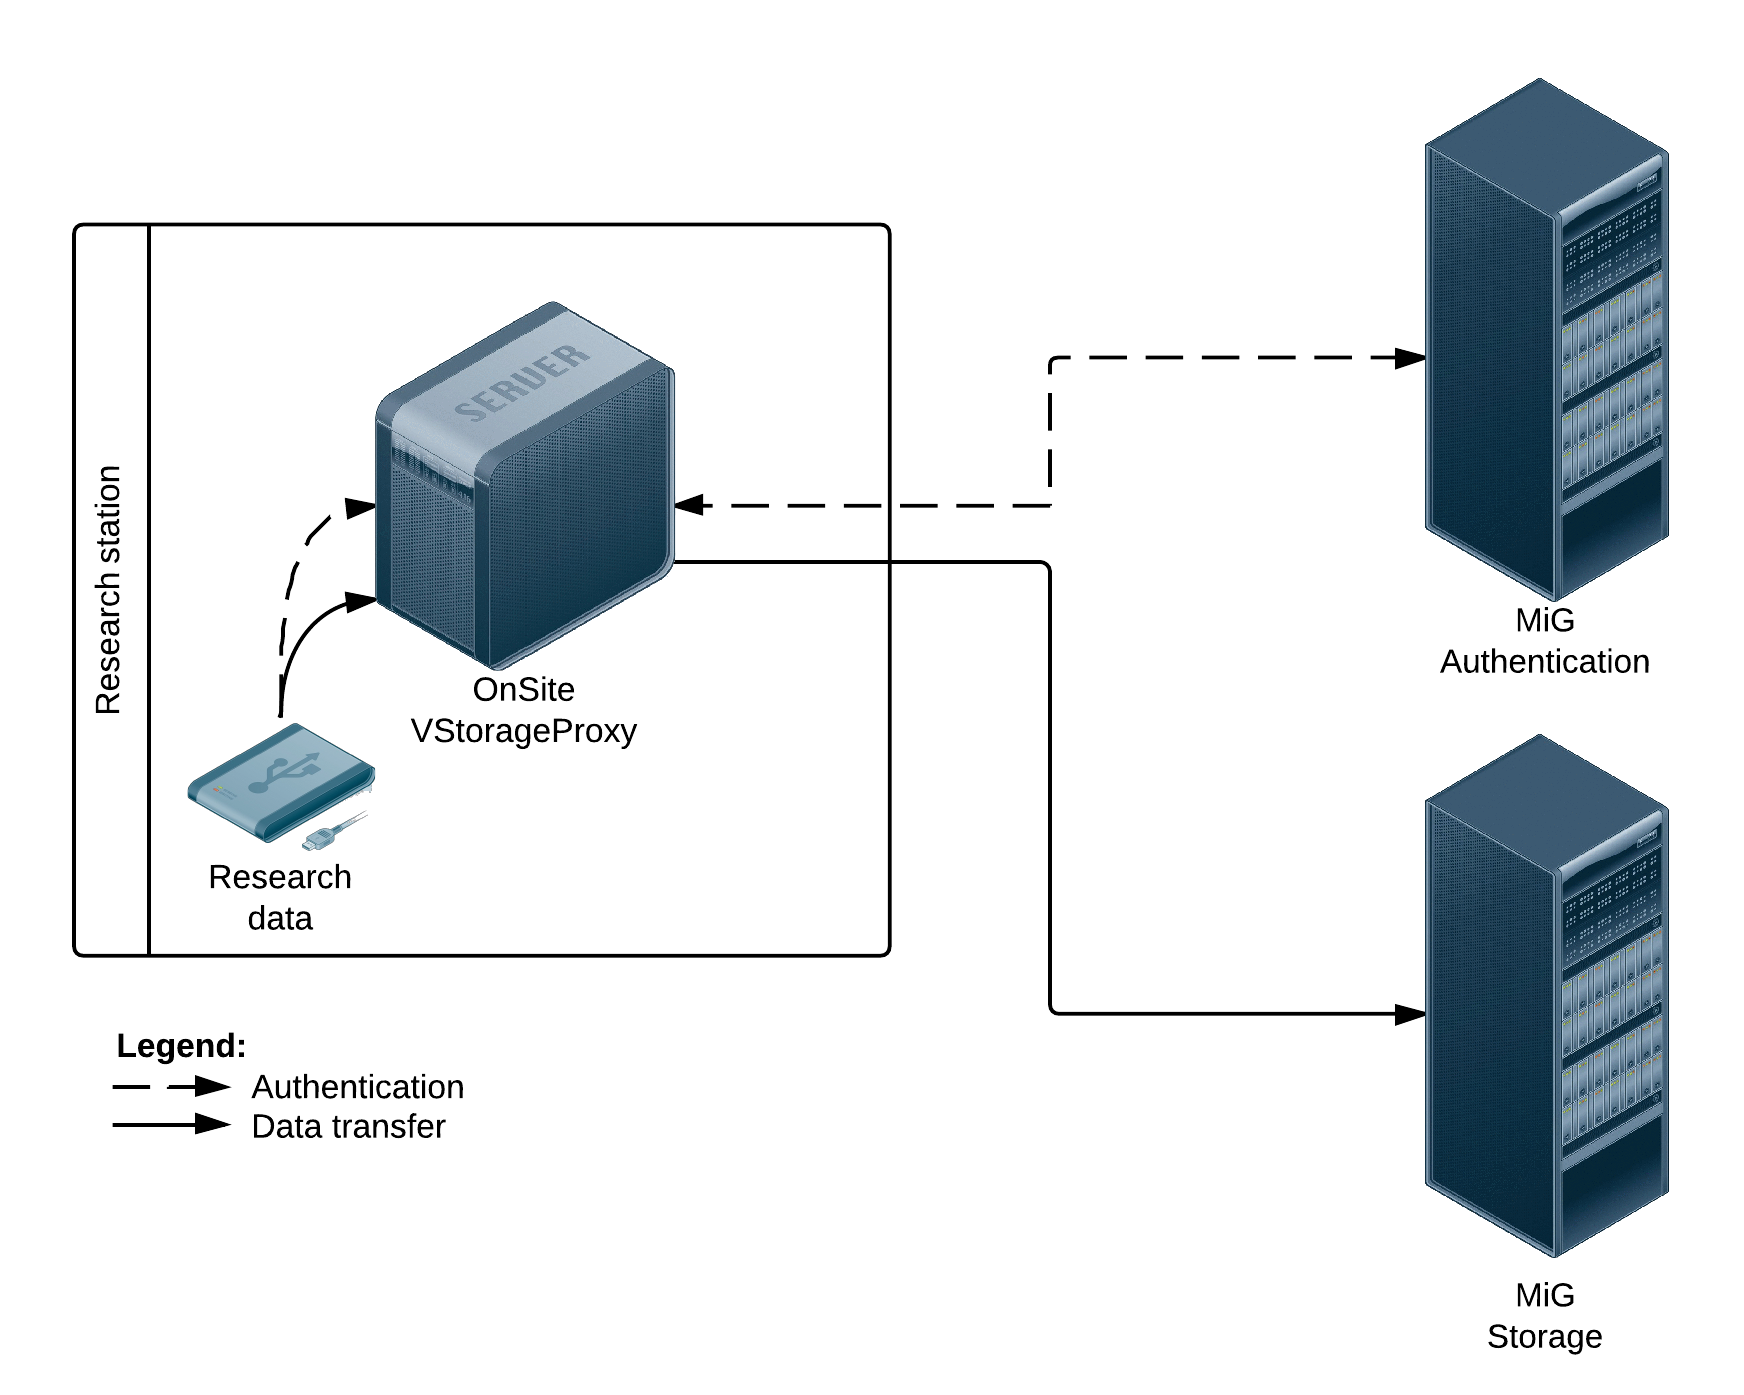
\includegraphics[width=0.8\textwidth]{diagram-design}
\caption{The overall design}
\label{fig:overall_design}
\end{figure}

Mainly three entites are envolved, the user and his temporary storage
device, the onsite proxy and the MiG central servers. The user interacts with
the onsite device, which in turn interacts with MiG to authenticate the user
and later on transfer the dropped of data.

The user should have the least of responsibilities, while the proxy has the
responsibility to authenticate and transfer, while MiG carries the
responsibility to store the data.

\begin{figure}[h]
\centering
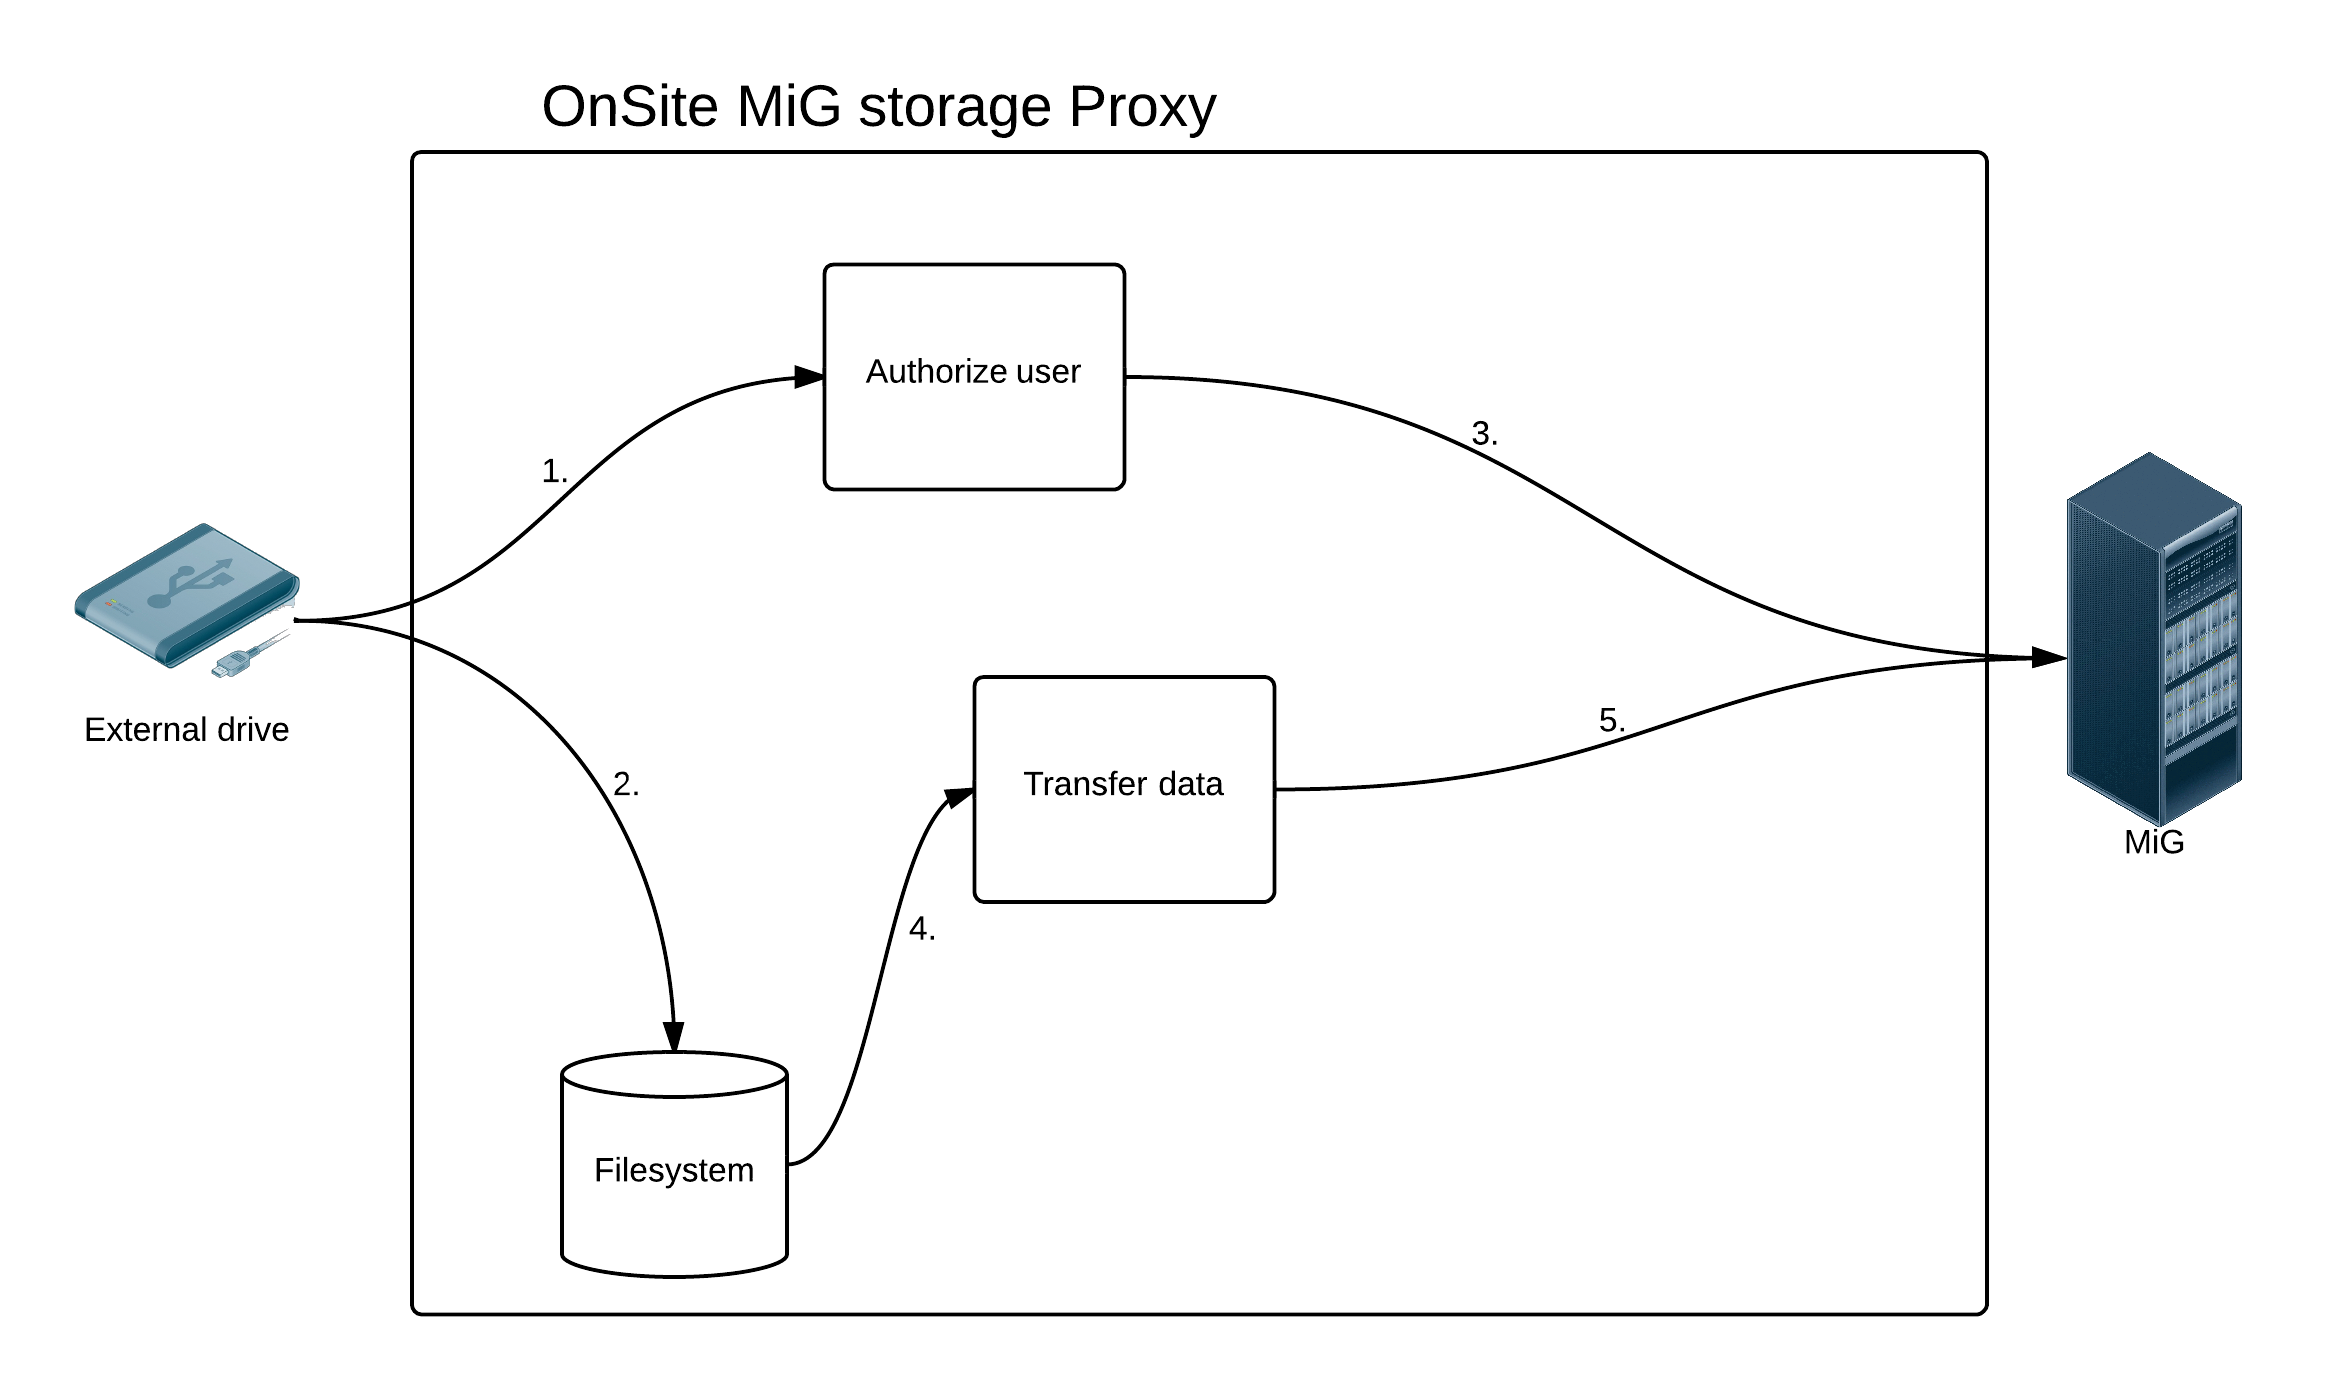
\includegraphics[width=0.8\textwidth]{MiG_ProxyBox}
\caption{The components of the onsite proxy}
\label{fig:proxy_components}
\end{figure}

\subsection{Protocol design}
The protocol for the operation of the solution, is described below in broad
terms, all relevant discussion of choices and so forth, has been put in the
relevant parts.

The way the proxy solution handles its overall task, is broken into the
components shown above. These tasks involve collaboration between one
another and dependencies on external parties.

When a user first connects their storage device, the proxy looks up their
personal certificate, and asks for a password to be able to connect to MiG. A
connection is then established and maintained for the length of the session.

Secondly data is lifted from the device, and stored temporarily on the proxy
machine. When this process has a go-signal from the ``authentication''-system, 
it starts transferring data, via the established connection.

